\documentclass[../../main.tex]{subfiles}
\begin{document}
\begin{refsection}
\chapter{深度卷积网络:实例探究}
% Deep convolutional models: case studies
\section{为什么要进行实例探究?}
% Why look at case studies?
\noindent 本节大纲:
\begin{enumerate}
    \item Classic Net
    \begin{enumerate}
        \item LeNet-5
        \item AlexNet
        \item VGG
    \end{enumerate}
    \item ResNet
    \item Inception Neural Network。
\end{enumerate}

组件、网络结构、超参数都可以参考别人的优秀案例,而且跨领域参考也有效。
\section{经典网络}

\subsection{LeNet-5}

\subsection{AlexNet}

\subsection{VGG-16}

\section{残差网络 (ResNets)\cite{arXiv:1512.03385}}
% Residual Networks (ResNets)
\index{ResNet@ResNet 残差网络}
在理论上,随着网络深度的增加,性能应该越来越好,但因为存在梯度消失/爆炸问题、网络退化,网络达到一定深度后,性能反而下降,\textbf{残差网络(Residual Network,简称为 ResNet)}可以有效解决这个问题。

\begin{figure}[H]
    \centering
    \begin{tikzpicture}[
        -latex,
        node distance=15mm,
        block/.style={draw, rectangle, minimum height=2cm, minimum width=5mm},
        skip path/.style={to path={-- ++(0, 14mm) -| (\tikztotarget)}},
    ]
      \node (a0) at (0,0) {\(a^{[l]}\)};
      \node[block,right=of  a0] (b1) {};
      \node[block,right=of  b1] (b2) {};
      \node[right=of  b2] (a2) {\(a^{[l+2]}\)};
      \draw (a0) -- (b1);
      \draw (b1) -- (b2) node[above,midway]{\(a^{[l+1]}\)};
      \draw (b2) -- (a2);
      \draw[skip path, red] ($(a0)!.5!(b1)$) to (b2.north);
  \end{tikzpicture}
\end{figure}

残差网络由许多残差块\textbf{残差块(Residual block)}组成。残差块通过\textbf{捷径(Short cut)}或者称\textbf{跳远连接,Skip connections},将\(a^{[l]}\)跳过第\(l+1\)层,添加到\(z^{[l+2]}\),如果原来的普通网络中\(
a^{[l+2]} = g(z^{[l+2]})
\),
使用了跳远连接后\[
    a^{[l+2]} = g(z^{[l+2]} + a^{[l]})
\]

\section{残差网络为什么有用?}
% Why ResNets work?
残差网络为什么有用?现在没有很好的解释,但是可以说明的是残差网络不会降低网络表现,随着网络深度增加性能变差(网络退化)的问题。

首先,对于某个问题,应该是存在最优网络层次的,如果继续增加将会产生冗余网络层,那么我们希望这些冗余层能自动消失:完成\textbf{恒等映射(identity map)},保证经过该恒等层的输入和输出完全相同,但是非线性的激活函数很难完成这一点,残差块跳远连接可以很容易做到恒等映射。

比如一个残差块:
\begin{align*}
    a^{[l+2]} & = g(z^{[l+2]}+a^{[l]})                    \\
              & = g(W^{[l+2]}a^{[l+1]}+b^{[l+2]}+a^{[l]})
\end{align*}
只要权重和偏置接近零,即可实现恒等映射\(a^{[l+2]} = a^{[l]}\),因此这两层外的残差块相当于没有,肯定不会降低网络性能。

\begin{remark}
    虽然\(W^{[l+2]}\)接近零,但因为有相加的一项\(a^{[l]}\),并不会造成梯度消失。
\end{remark}

实现时需要注意的是如果\(a^{[l]}\)与\(a^{[l+2]}\)形状不同,可以使用填充、截断,或者引入一个\(W_s\),使得\(W_sa^{[l]}\)与\(a^{[l+2]}\)形状相同,它可以是模型参数,也可以是一个固定矩阵。

\begin{figure}[p]
    \centering
    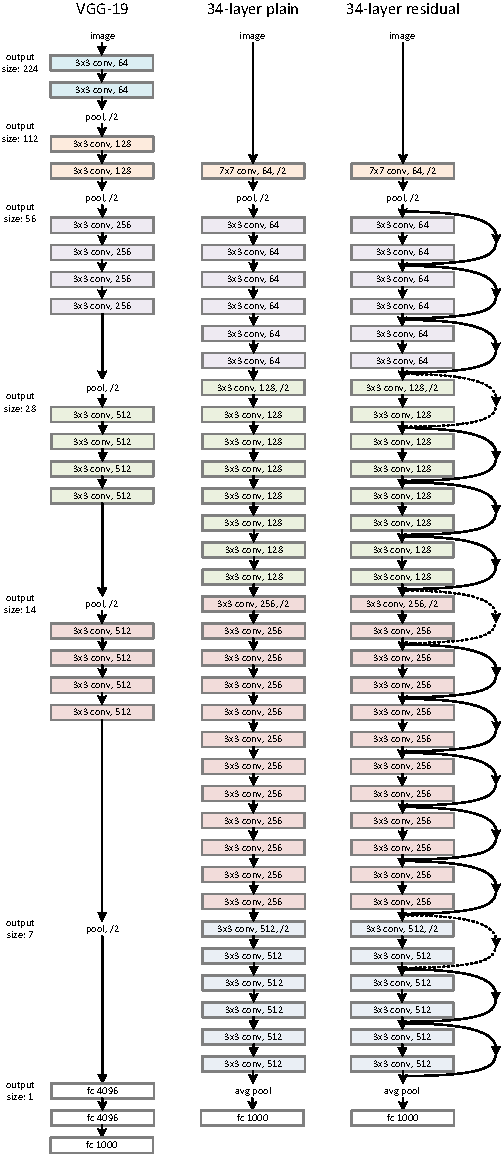
\includegraphics[height=\textheight]{./img/resnet-arch.pdf}
    \caption{ResNet 论文中的示例架构}
\end{figure}

\section{网络中的网络以及 1×1 卷积}
% Network in Network and 1×1 convolutions
1×1卷积在二维时没有什么用,但在三维时用处很大,因为它不会改变数组和高度和宽度,可以减少或增加通道数,这一点十分有用。这种方法通常称为1×1卷积,有时也被称为\textbf{Network in Network}。

\section{谷歌 Inception 网络简介}
% Inception network motivation
构建卷积层时,我们要决定过滤器的大小、考虑是否添加池化层,\textbf{Inception Net}则代替人工来确定卷积层中的滤波器尺寸与类型,或者确定是否需要创建卷积层或池化层,它将多种选择堆叠在一层中,让模型去学习。

如图\ref{fig:inception-naive-module},它将输入经过了\(1×1, 3×3, 5×5\)三个过滤器和一个最大池化,并使用same padding(包括池化)来保证这些操作的输出的高、宽相同,将这些输出堆叠在一起作为这一层的输出。
\begin{figure}[htbp]
    \centering
    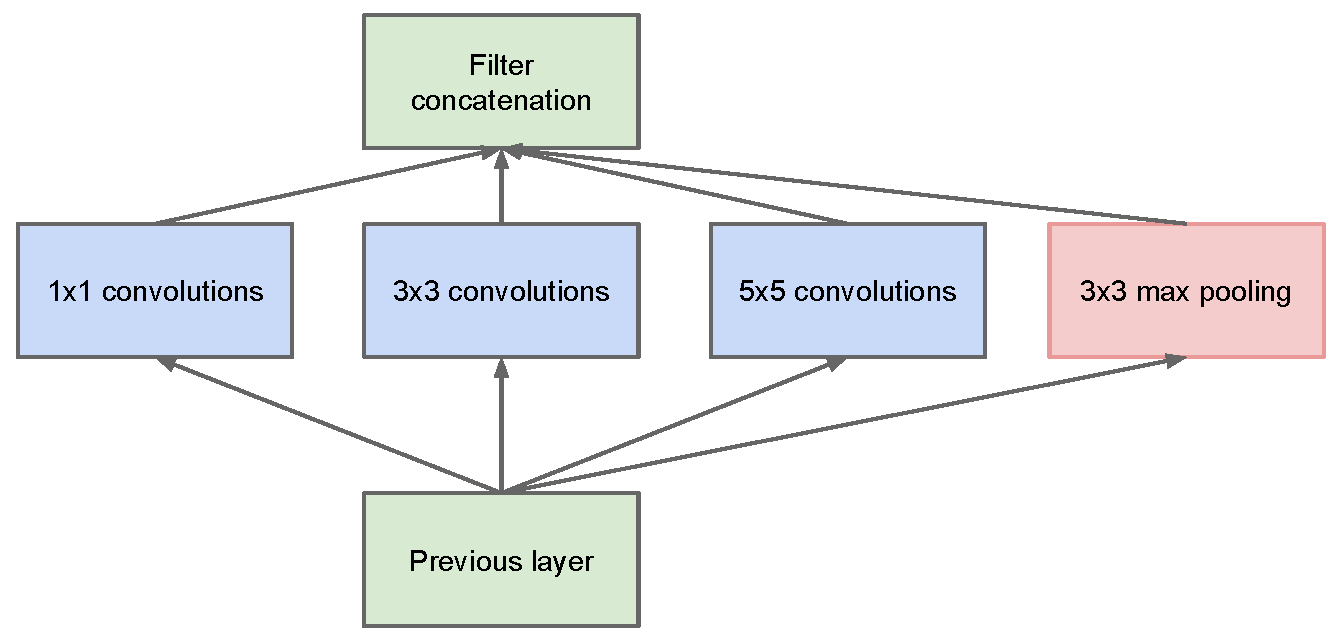
\includegraphics[width=0.75\columnwidth]{./img/inception-naive-module.pdf}
    \caption{Inception Naive Module}
    \label{fig:inception-naive-module}
\end{figure}
这样的网络表现确实非常好,但很明显网络架构因此变得更加复杂,对算力的要求更高,Inception使用\textbf{瓶颈层(Bottleneck layer)}大幅度降低了计算成本。

简言之,如此大的输入与\(3×3, 5×5\)的过滤器做卷积操作的计算量巨大,Inception引入了瓶颈层,即图\ref{fig:inception-module}中在与\(3×3, 5×5\)过滤器作卷积操作前,先与\(1×1\)做的卷积操作(最大池化后的\(1×1\)是为了调整通道数)。使用这样的方法计算量大致能降低到原来的10\%。
\begin{figure}[htbp]
    \centering
    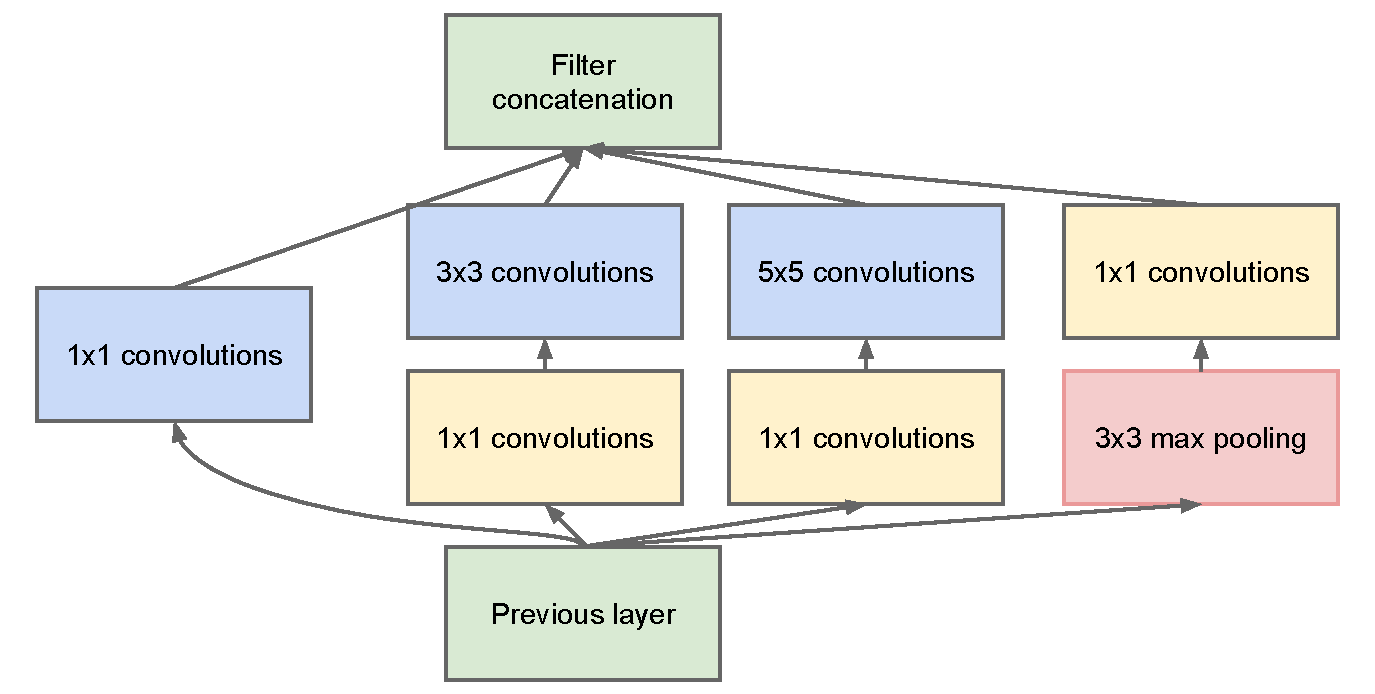
\includegraphics[width=0.7\columnwidth]{./img/inception-module.pdf}
    \caption{Inception Module}
    \label{fig:inception-module}
\end{figure}

瓶颈层尽管压缩了信息,但只要合理构建瓶颈层,就可以既显著缩小计算规模,又不会降低网络性能。

\section{Inception 网络}
% Inception network
完整的Inception中还需要注意的是,网络中有多个分支都是Softmax的输出层,可以用来参与特征的计算及结果预测,起到调整并防止发生过拟合的效果。

Inception也在不断的改进,有多个版本,有的还结合了残差网络,但基本的思想与这个一致。
\begin{figure}[p]
    \centering
    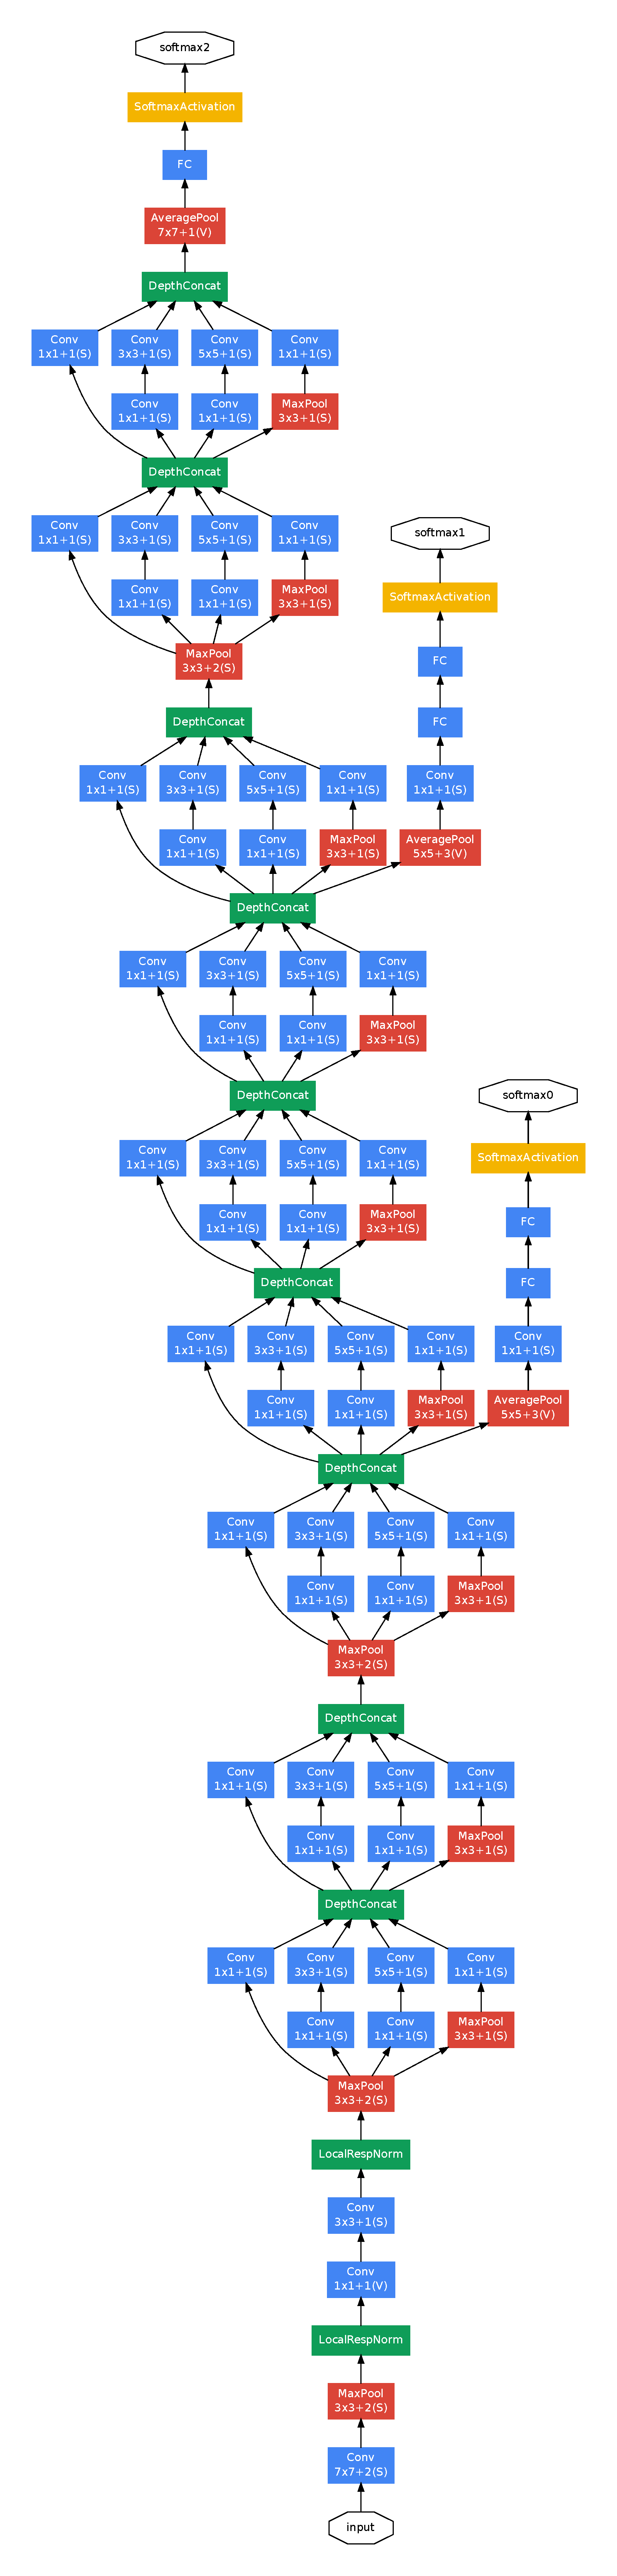
\includegraphics[height=\textheight]{./img/inception-overall.pdf}
    \caption{完整的Inception网络}
\end{figure}

\section{使用开源的实现方案}
% Using open-source implementations
很多神经网络复杂细致,并充斥着参数调节的细节问题,因而很难仅通过阅读论文来重现他人的成果。想要搭建一个同样的神经网络,查看开源的实现方案会快很多。

\section{迁移学习}
% Transfer Learning
迁移学习是非常值得你考虑的,除非你有一个极其大的数据集和非常大的计算量预算来从头训练你的网络。

根据自己的数据量,选择冻结预训练模型的层数,或者将其作为初始参数继续训练。

\section{数据增强}
% Data augmentation

\section{计算机视觉现状}
% The state of computer vision
通常,学习算法有两种知识来源:被标记的数据和手工工程。\textbf{手工工程(Hand-engineering,又称 hacks)}指精心设计的特性、网络体系结构或是系统的其他组件。手工工程是一项非常重要也比较困难的工作。在数据量不多的情况下,手工工程是获得良好表现的最佳方式。正因为数据量不能满足需要,历史上计算机视觉领域更多地依赖于手工工程。近几年数据量急剧增加,因此手工工程量大幅减少。

在模型研究或者竞赛方面,有一些方法能够有助于提升神经网络模型的性能:
\begin{itemize}
    \item 集成(Ensembling):独立地训练几个神经网络,并平均输出它们的输出;
    \item Multi-crop at test time:将数据扩增应用到测试集,对结果进行平均。
\end{itemize}
但是由于这些方法计算和内存成本较大,一般不适用于构建实际的生产项目。

\printbibliography[heading=subbibliography]
\end{refsection}
\end{document}